% ==============================================================================
\chapter{Simulation and reconstruction software frameworks}
\label{sec:Software}
%==============================================================================    

Simulation tools have a crucial role in the development and also
understanding of the performance of semiconductor devices. The
simulations are validated with the data and used to predict the
performance of small-pitch pixels for which data is not yet available.

This chapter describes the simulation tools used to understand the
performance of Timepix3 devices. The reconstruction software, used for
both data and simulation, is also presented.

%% --------------------------------------------- %%
\section{\textsc{Geant4}}\label{sec:Silicon_Geant4}

\textsc{Geant4}~\cite{Agostinelli:2002hh}, as an object-oriented
simulation toolkit implemented in the C++ programming language, is
widely used in high energy, nuclear and accelerator physics, medical
and space sciences. As modern particle physics is going towards
large-scale detectors, more accurate simulations are needed in order
to understand the complex situations. \textsc{Geant4} provides
software components which can be used to study basic phenomena,
geometries and full-scale detector simulations for
experiments. \textsc{Geant4} simulations take into account parameters
such as: the geometry of the system, the materials involved, the
fundamental particles, the generation of primary particles, the
tracking of particles through materials and external electromagnetic
fields, the physics processes involved in the possible interaction of
the particles with the materials they are passing through, the
response of sensitive components. The simulations of the interaction
between the particles and materials are mostly validated with data. In
this thesis, all the studies using \textsc{Geant4} are done with
version 10.1.2.

\textsc{Geant4} provides physics models for different type of
interactions called \textit{physics lists}. The \textit{emstandard}
physics lists provide the electromagnetic interactions of photons and
charged particles with matter and is suited for the simulation of
ionisation, bremsstrahlung, gamma conversion and other electromagnetic
interactions of particles with energies from $1\,\kev$ up to
$10\,\pev$~\cite{Apostolakis2009859}. This physics list is commonly
used for the simulation of the energy loss in pixel detectors.

\textsc{Geant4} provides as well the Photo-Absorption Ionisation (PAI)
model~\cite{Apostolakis:2000yu} for the precise simulation of
ionisation energy loss by relativistic charged particles in very thin
absorbers. Since in very thin sensors the Landau model is not suitable
(see \cref{sec:landau}), the PAI model is based on the
photo-absorption cross-section tables obtained by experimental
data. In practice several classes are used to calculate the integral
ionisation cross-section, the mean number of ionising collisions as
well as the mean ionisation energy loss for the selected material and
the given Lorentz factor.



\cref{fig:BichselVSG4} compares the energy loss due to ionisation in
$50\,\micron$ and $450\,\micron$ thick silicon sensors for different
\textsc{Geant4} physics lists and the Bichsel parametrisation
(see~\cref{sec:bichsel}). For the $50\,\micron$ thick sensor, the
\textit{emstandard\_opt3} physics list gives a reasonable value for
the most probable value ($\Delta_p$) but the width ($w$) of the
distribution is more narrow than the Bichsel distribution. The PAI
model shows a very good agreement with the Bichsel model. For the
thick sensor of $450\,\micron$, both PAI and emstandard\_opt3 physics
lists show similar distributions as the Bichsel model.

The energy deposition given by the PAI model is very close to the one
calculated by Bichsel especially for the fluctuations around the most
probable value and for very thin sensors. For this reason, the PAI
model is chosen to be used later for the simulations even though it
requires more computation power.
 
\begin{figure}[htbp] \centering
  \begin{subfigure}[b]{0.45\textwidth}
    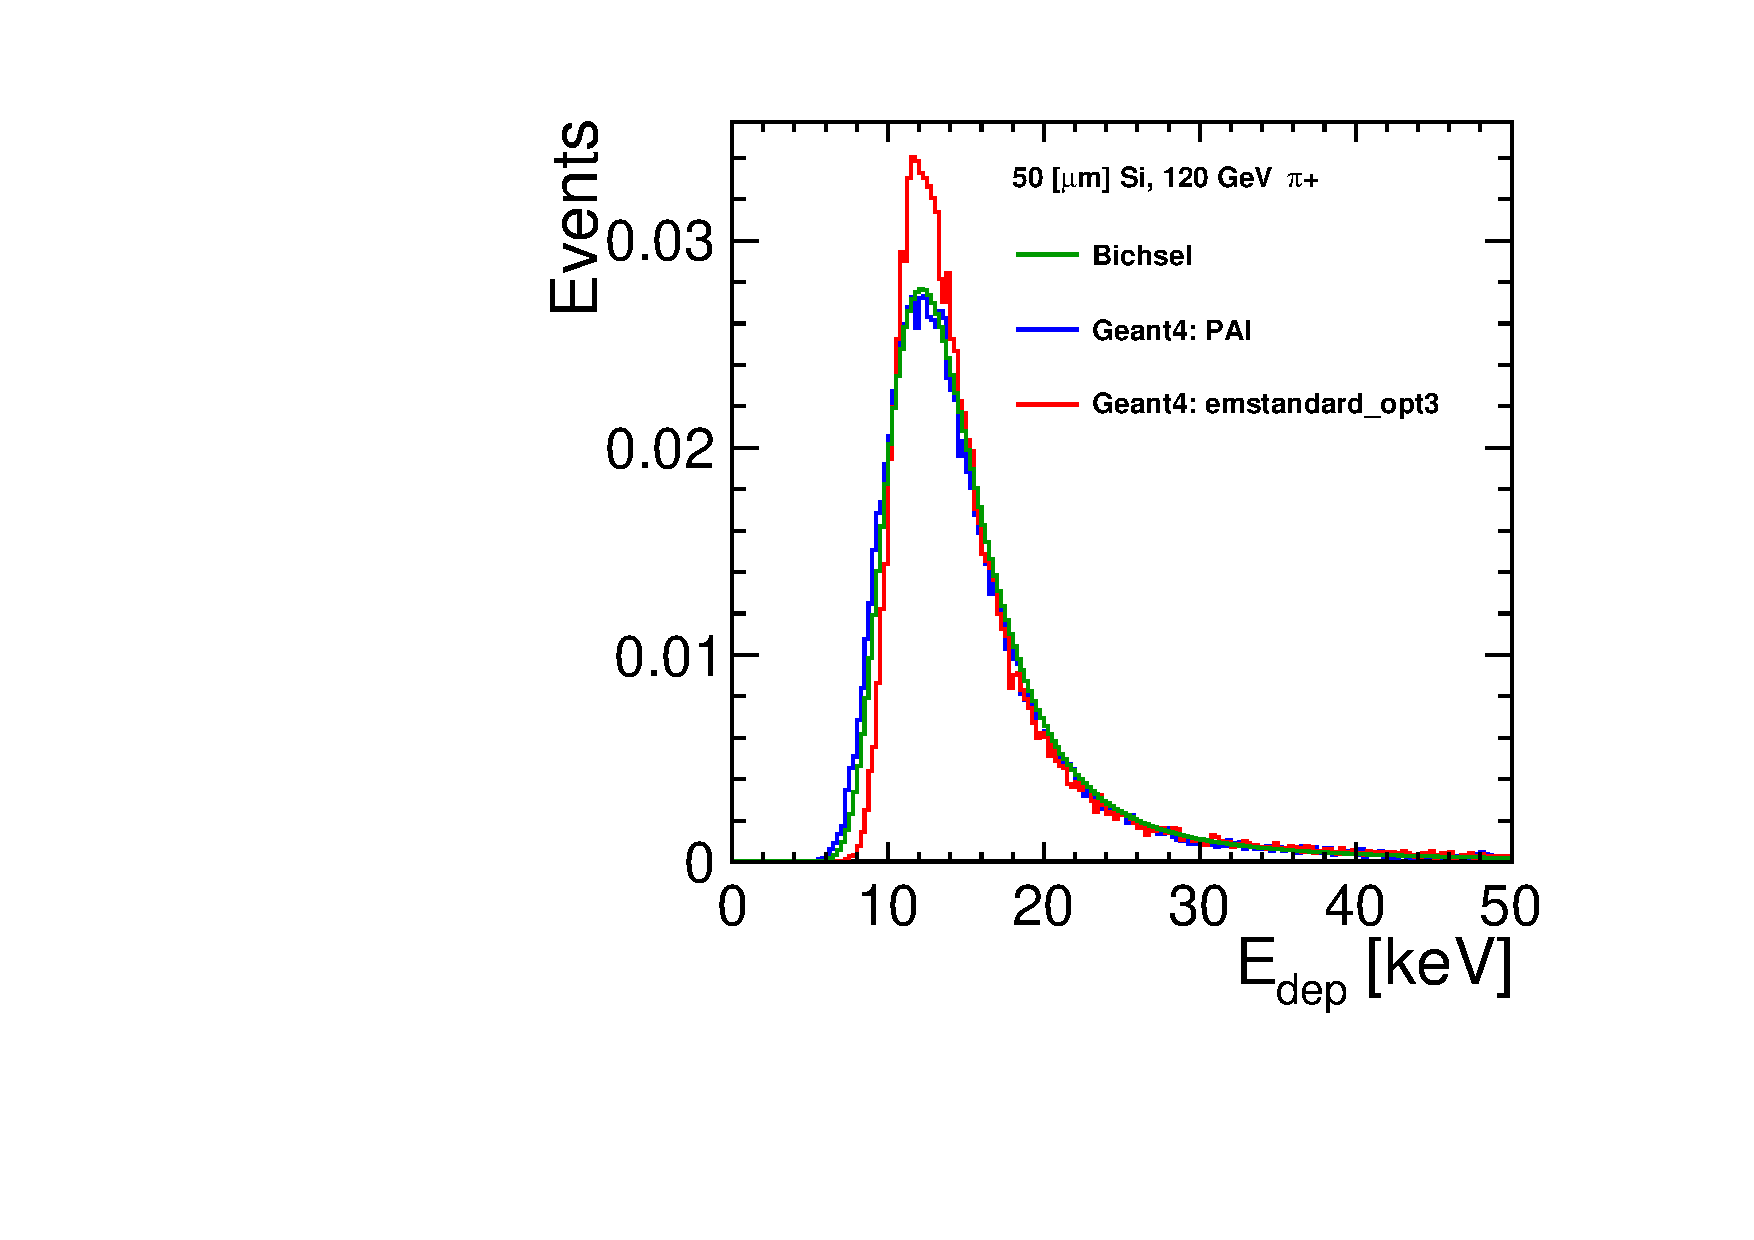
\includegraphics[width=\textwidth]{figures/ChargeSharing/50um_bichsel_physicsLists.pdf}
    \caption{}
  \end{subfigure} \hfill
  \begin{subfigure}[b]{0.45\textwidth}
    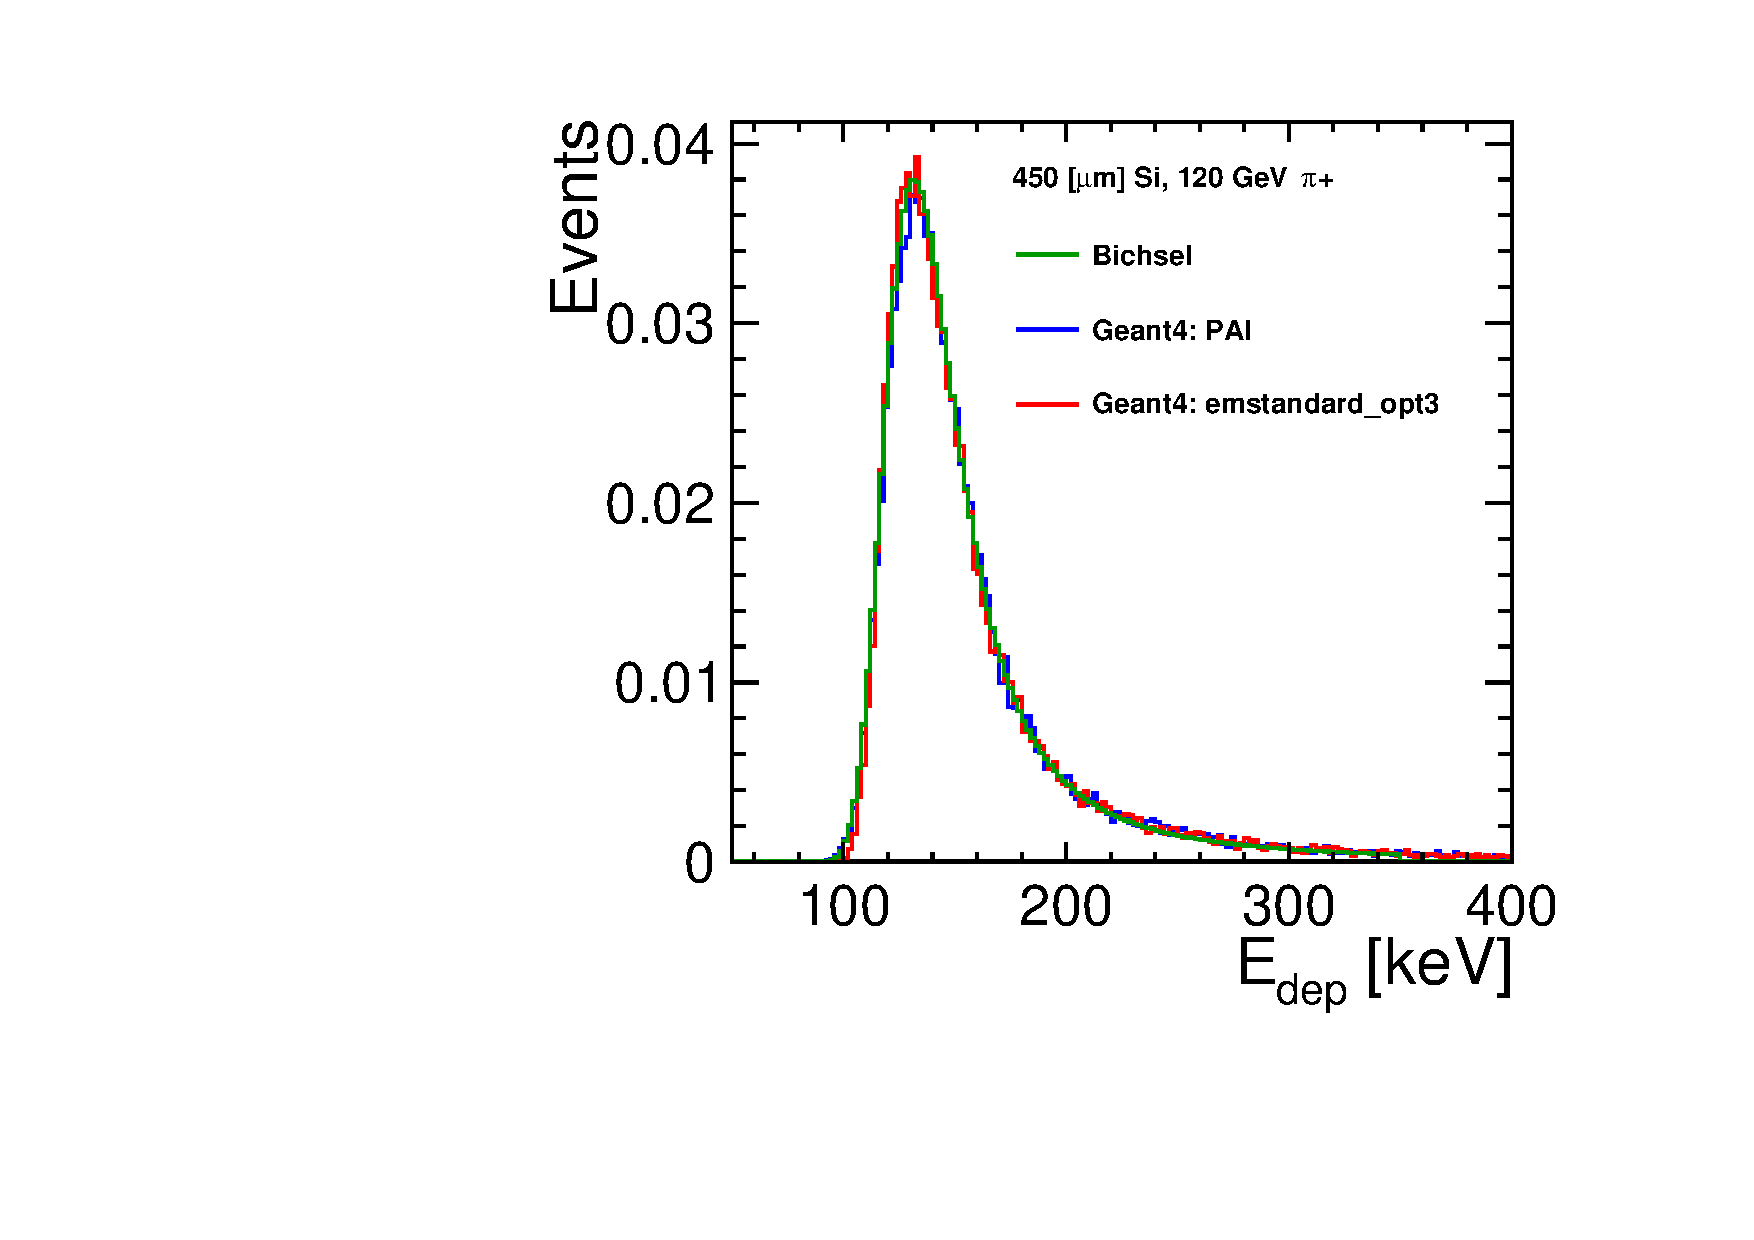
\includegraphics[width=\textwidth]{figures/ChargeSharing/450um_bichsel_physicsLists.pdf}
    \caption{}
  \end{subfigure}
  \caption{Energy-loss distribution in (a) $50\,\micron$ and (b)
    $450\,\micron$ thick silicon sensors by $120\,\gev$ $\pi^{+}$
    comparing the Bichsel model and \textsc{Geant4} using the PAI and
    the emstandard\_opt3 physics lists.}
  \label{fig:BichselVSG4}
\end{figure}

%% --------------------------------------------- %%
\section{AllPix simulation framework}
\label{sec:AllPix}

AllPix~\cite{allpix} is a \textsc{Geant4}-based simulation software
framework. It is written in C/C++ and provides a flexible interface to
define any pixel detector geometry to simulate pixelated sensors and
readout chips.

\textsc{Geant4} provides the simulation of particles through the
matter: it calculates the position of the hits (or the Monte Carlo
Truth position) considering the multiple scatterings and the energy
deposition in the sensitive volumes (sensors). The software user
defines the semiconductor physics and readout chip properties in a
digitiser as described here below.

\cref{fig:TPX3TelescopeAllpix} shows an example of the simulation for
the Timepix3 telescope (described in \cref{ch:Telescope}) in AllPix
with the device under test (DUT) in the middle of the rotated telescope
planes.

\begin{figure}[htbp]
  \centering
  \begin{tikzpicture}
    \node[anchor=south west,inner sep=0] (image) at
    (0,0){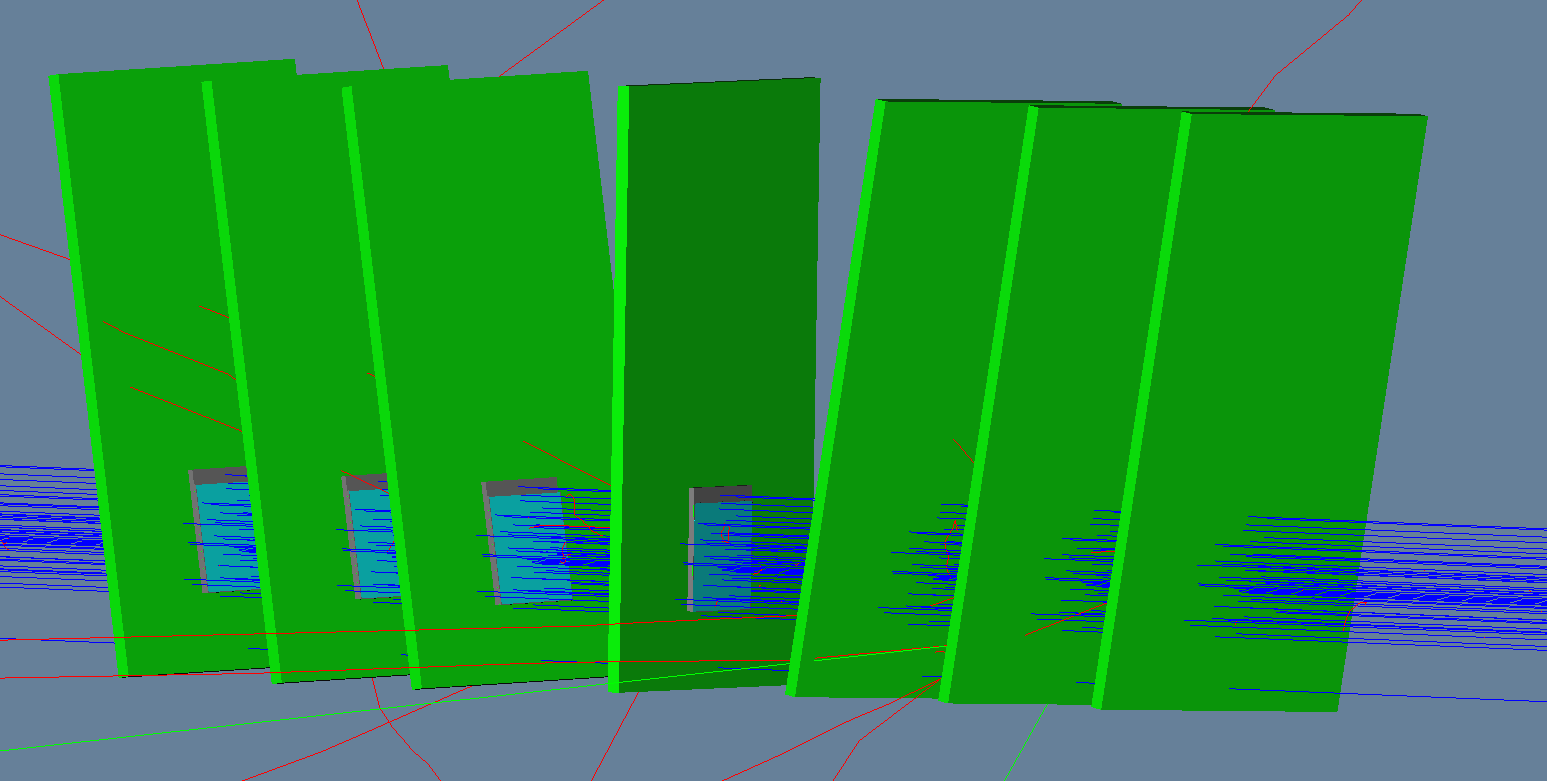
\includegraphics[width=0.8\textwidth]{figures/ActiveEdge/Allpix_telescope_withParticles.png}};
    \begin{scope}[x={(image.south east)},y={(image.north west)}]
      \node[above, color=white] at (0.45, 0.65) {\textbf{DUT}};
    \end{scope}
  \end{tikzpicture}
  \caption{Simulation of the Timepix3 telescope with AllPix.}
  \label{fig:TPX3TelescopeAllpix}
\end{figure}

%% --------------------------------------------- %%
\subsection{Coordinate system}

The convention used for the pixel detectors (in AllPix but also the
reconstruction software as described in \cref{sec:recoSoft}) for a
Timepix3-like matrix of $256\times256$ pixels is shown in
\cref{fig:coordinateSystem}. The pixel coordinates (X, Y) and the
\textcolor{blue}{local coordinates (x, y) in millimeters} of the
center of the pixels in the corners of the matrix are shown. In this
convention we are looking from the sensor side with the periphery on
the top.

\begin{figure}[htbp]
  \centering
  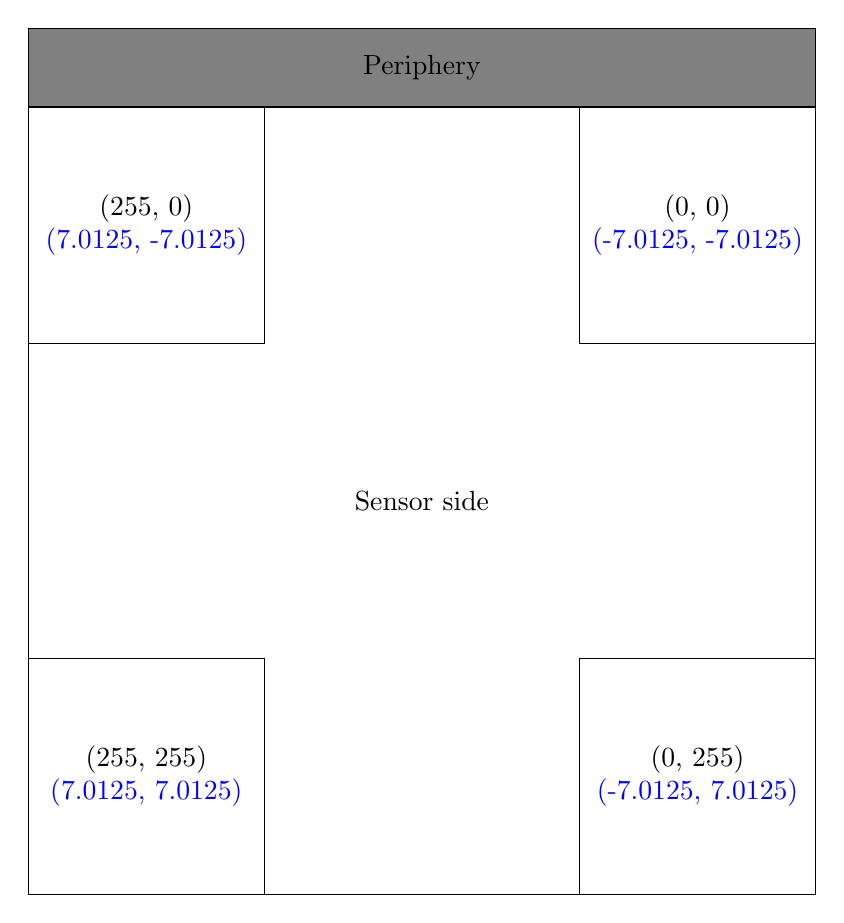
\begin{tikzpicture}
    \begin{scope} 

      \draw (0, 0) rectangle (10, 10) node[pos=.5] {Sensor side};
      \draw[fill=gray] (0, 10) rectangle (10, 11) node[pos=.5]
      {Periphery};

      \draw (0, 10) rectangle (3, 7) node[align=center, pos=.5] {(255, 0) \\ \textcolor{blue}{(7.0125, -7.0125)}};
      \draw (7, 10) rectangle (10, 7) node[align=center, pos=.5] {(0, 0) \\ \textcolor{blue}{(-7.0125, -7.0125)}};
      
      \draw (0, 0) rectangle (3, 3) node[align=center, pos=.5] {(255,
        255) \\ \textcolor{blue}{(7.0125, 7.0125)}};
      \draw (7, 0) rectangle (10, 3) node[align=center, pos=.5] {(0, 255) \\ \textcolor{blue}{(-7.0125, 7.0125)}};
      % \draw[help lines,xstep=.1,ystep=.1] (0, 0) grid (10,10);
      % \foreach \x in {0,1,...,9} { \node [anchor=north] at (\x/10,0) {0.\x}; }
      % \foreach \y in {0,1,...,9} { \node [anchor=east] at (0,\y/10)
      %   {0.\y}; }

    %   \draw[step=2cm,color=gray] (-5, -5) grid (5, 5);
    %   \matrix[matrix of nodes,nodes={inner sep=0pt,text width=2cm,align=center,minimum height=2cm}]{
    %     {(255, 0) \\ \textcolor{blue}{(7.0125, -7.0125)}} & &  & {(0,0) \\ \textcolor{blue}{(-7.0125, -7.0125)}} \\
    %     &  &  &  \\
    %     &  &  &  \\
    %     {(255, 255) \\ \textcolor{blue}{(7.0125, 7.0125)}} &  &  & {(0, 255) \\ \textcolor{blue}{(-7.0125, 7.0125)}} \\};
    \end{scope}  
  \end{tikzpicture}
  \caption{The coordinates system for a matrix of $256\times256$
    pixels. The pixel coordinates (X, Y) and the
    \textcolor{blue}{local coordinates (x, y) in millimeters} of the
    center of the pixels in the corners of the matrix are shown. In
    this convention, we are looking from the sensor side with the
    periphery on the top.}
  \label{fig:coordinateSystem}
\end{figure}
%% --------------------------------------------- %%
\subsection{Geometry of the pixel detector}

In AllPix, the pixel detector geometry can be defined by the pitch
size, the thickness of the sensor and the readout chip, the PCB
properties, the mechanical support and other geometry properties
related to an assembly. These parameters are usually defined in an XML
file format called the \texttt{pixeldetector.xml}. Each detector is
identified by a unique ID. This facilitates the running of the
simulation with different parameters by only changing the
\texttt{pixeldetector.xml} file without any need of re-compiling the
code. It is also possible to define the parameters of the digitiser in
this XML file.
%% --------------------------------------------- %%
\subsection{Geometry of the simulation scenario}

The simulation scenario is defined in the file \texttt{macro.in}. The
position of the detectors in the space is specified by the coordinates
(x, y, z) and the rotations around the x, y and z axes of the centre
of the detectors. The physics list used by \textsc{Geant4} is
specified. The General Particle Source (GPS), which is the
\textsc{Geant4} toolkit for Monte-Carlo of the high-energy particle
transport is also described in the macro. The particle type, the beam
energy, the position and distributions are customisable. The
simulation is done based on frames.

Visualisation parameters are also given in the macro. Open
Inventor~\cite{OpenInventor} can be, for example, used to visualise
the simulation scenario and also the particle tracks in the detectors.

%% --------------------------------------------- %%
\subsection{Digitisation}
\label{sec:allpix_digitisation}

\textsc{Geant4}, for each simulation step (\texttt{G4Step}) through
the matter, provides the energy deposited in the sensitive
material. The step length can be customised. For thin sensors
simulations, a step of $2\,\micron$ is selected and provides a precise
energy deposition. The semiconductor physics in a Silicon detector is
then defined in the digitiser. The drift and diffusion are performed
at each step (using \cref{eq:sigmaDiffusion}) to simulate the
electron-hole pair movement in the electric field. The digitiser also
defines the parameters of the readout chip. The electronic noise is
added and the chip threshold are applied to the hits. The hit energy
is converted to the digital value TOT (time-over-threshold) using the
readout ASICs calibrations.

\cref{fig:digitisation} schematically illustrates the digitisation in
a sensor. Each \textsc{Geant4} step is shown in a circle. At each
step, the contribution of the diffusion is calculated in the hit and
its neighbouring pixels. For each pixel, all the contributions sum up
and the total charge deposited in a pixel is calculated.

\begin{figure}[htbp]
  \centering
  \begin{tikzpicture}[node distance = 2.5cm, auto]
    \begin{scope}[x={(image.south east)},y={(image.north west)}]

      \draw[thick] (0.2, 0.6) -- (0.8, 0.6);
      \draw[thick] (0.2, 0.2) -- (0.8, 0.2);

      \draw[thick] (0.2, 0.2) -- (0.2, 0.6);
      \draw[thick] (0.8, 0.2) -- (0.8, 0.6);  

      \draw[thick] (0.4, 0.2) -- (0.4, 0.6);  
      \draw[thick] (0.6, 0.2) -- (0.6, 0.6);  

 


      \draw[green, thick] (0.45, 0.2) circle (0.5mm);
      \node[right, color=green] at (0.45, 0.22) {Step 1};
      \draw[green, thick] (0.45, 0.2) -- (0.36, 0.6);  
      \draw[green, thick] (0.45, 0.2) -- (0.54, 0.6);
      \draw[green, thick, <->] (0.36, 0.62) -- (0.54, 0.62);
      \node[above, color=green] at (0.36, 0.62) {$\sigma_{1}$};

      \draw[red, thick] (0.473, 0.3) circle (0.5mm);
      \node[right, color=red] at (0.473, 0.32) {Step 2};
      \draw[red, thick] (0.473, 0.3) -- (0.403, 0.6);
      \draw[red, thick] (0.473, 0.3) -- (0.543, 0.6);
      \draw[red, thick, <->] (0.403, 0.64) -- (0.543, 0.64);
      \node[above, color=red] at (0.403, 0.64) {$\sigma_{2}$};

      \draw[cyan, thick] (0.5, 0.4) circle (0.5mm);
      \node[right, color=cyan] at (0.5, 0.42) {Step 3};
      \draw[cyan, thick] (0.5, 0.4) -- (0.45, 0.6);
      \draw[cyan, thick] (0.5, 0.4) -- (0.55, 0.6);
      \draw[cyan, thick, <->] (0.45, 0.66) -- (0.55, 0.66);
      \node[above, color=cyan] at (0.45, 0.66) {$\sigma_{3}$};

      \draw[purple, thick] (0.525, 0.5) circle (0.5mm);
      \node[right, color=purple] at (0.525, 0.52) {Step 4};
      \draw[purple, thick] (0.525, 0.5) -- (0.495, 0.6);
      \draw[purple, thick] (0.525, 0.5) -- (0.555, 0.6);
      \draw[purple, thick, <->] (0.495, 0.68) -- (0.555, 0.68);
      \node[above, color=purple] at (0.495, 0.68) {$\sigma_{4}$};

      \draw[blue, thick, ->] (0.4, 0.0) -- (0.6, 0.8);  
      \node[above, color=blue] at (0.6, 0.8) {MIP};
      \draw[black, thick, ->] (0.1, 0.2) -- (0.1, 0.6);  
      \node[left, color=black] at (0.1, 0.4) {E\textsubscript{field}};

      \node[below, color=black] at (0.3, 0.15) {Pixel 1};
      \node[below, color=black] at (0.5, 0.15) {Pixel 2};
      \node[below, color=black] at (0.7, 0.15) {Pixel 3};

      %% \node at (4.5,4) 
      %% {some text spanning three lines with automatic line breaks};

      %% \draw[help lines,xstep=.1,ystep=.1] (0, 0) grid (1,1);
      %% \foreach \x in {0,1,...,9} { \node [anchor=north] at (\x/10,0) {0.\x}; }
      %% \foreach \y in {0,1,...,9} { \node [anchor=east] at (0,\y/10) {0.\y}; }
    \end{scope}
  \end{tikzpicture}
  \caption{Illustration of the digitisation in a sensor. Each
    \textsc{Geant4} step (\texttt{G4Step}) is shown with a circle. The
    contribution of the diffusion ($\sigma_1$, $\sigma_2$, $\sigma_3$
    and $\sigma_4$) in the hit and its neighbouring pixels is
    calculated.}
  \label{fig:digitisation}
\end{figure}


%% --------------------------------------------- %%
%% --------------------------------------------- %%
\section{TCAD simulations}
\label{sec:TCAD}
Technology Computer-Aided Design (TCAD) as a powerful simulation tool
is used to optimise and develop semiconductor processing technologies
as well as the device operation~\cite{synopsysTCAD}. TCAD uses the
finite element method to numerically solve the solutions to the
physical partial differential equations in semiconductor, such as the
continuity and diffusion equations. This allows for the modeling of
the structural properties and the electrical behaviour of
semiconductor devices.

For this study Synopsys TCAD version I-2013.12 is used for several
purposes. First to understand the movement of charge carriers in
silicon and the coupling to the readout in as described in
\cref{sec:RamoTheorem}. Also it is used to simulate active-edge
devices and understand the measurements later in
\cref{ch:ActiveEdgeSensors}.
%% --------------------------------------------- %%

%% --------------------------------------------- %%
\section{Reconstruction and analysis software frameworks}
\label{sec:recoSoft}

The offline reconstruction of the test beam data is done using two
software frameworks. The EUTelescope software
package~\cite{Rubinskiy,EutelescopeWebsite} is used to reconstruct the
tracks from the telescope and extrapolate their positions on the
DUT. For the analysis of the DUT data, the python-based software
pyEudetanalysis is used (it can be found as a GitHub
directory~\cite{pyeudet}).

\subsection{EUTelescope}
\label{sec:EUTelescope}
The EUTelescope software is based on the ILCSoft
framework~\cite{Aplin:2009zz}. This latter provides the basic building
blocks such as the LCIO (Linear Collider Input Output) data model, the
geometry description toolkit GEAR and a modular application framework
for event analysis, called Marlin~\cite{Gaede:2006pj}.

A modular analysis and reconstruction chain can be defined using
Marlin processors. Each processor implements algorithms for specific
tasks. The input parameters for the algorithms can be configured and
loaded at runtime using \textit{steering files} in XML format. For
each event, the processors are called centrally by Marlin and this
scheme offers flexibility to the users.

EUTelescope framework, originally developed for the EUDET/AIDA pixel
beam telescope~\cite{Rubinskiy:2014kza}, provides Marlin processors
for the track reconstruction and data analysis of test beam
experiments. \cref{fig:EUTelescope_EUDET_pipeline} schematically shows
the analysis strategy in EUTelescope framework starting from the raw
data recorded during the test beam to finally particle tracks
reconstruction. Since each experiment has its own data format for the
DUT, the format converter is defined by the user. This makes the
framework more flexible for testing different chip families.

\begin{figure}[htbp]
  \centering
  \begin{tikzpicture}
    \node[anchor=south west,inner sep=0] (image) at
    (0,0){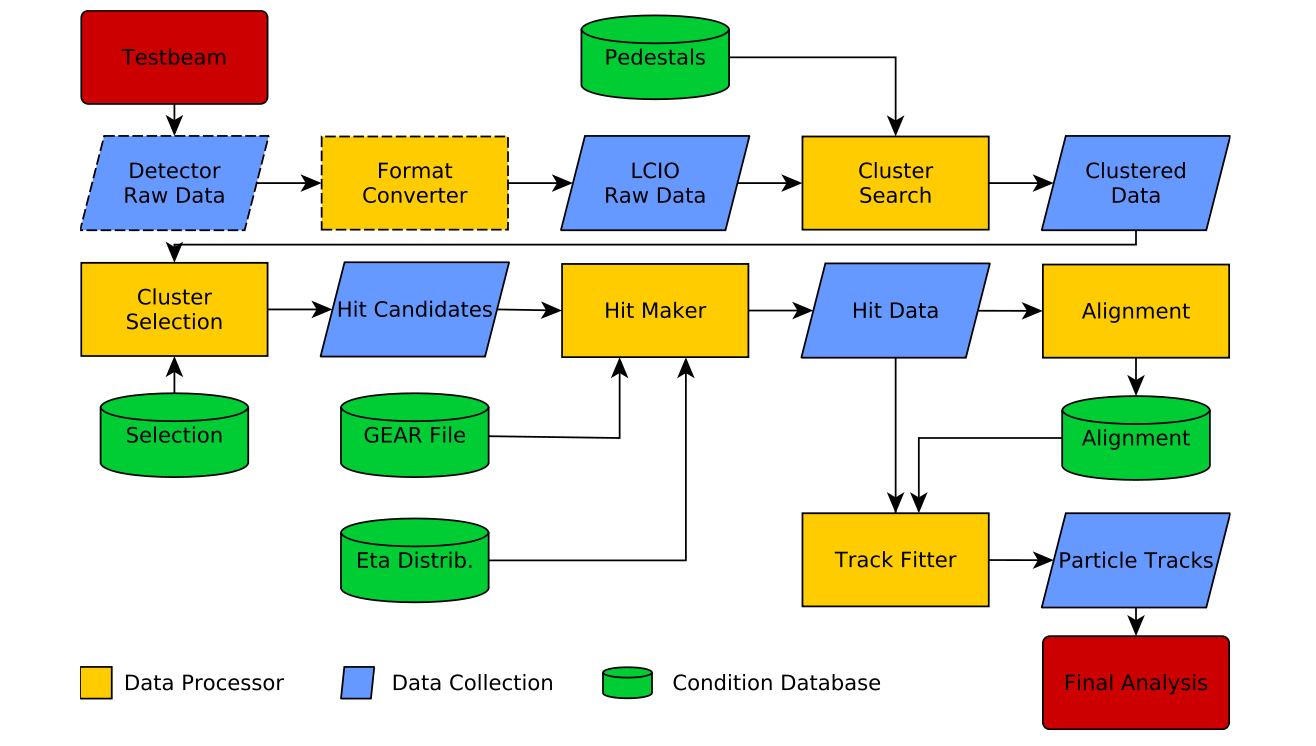
\includegraphics[width=0.8\textwidth]{figures/Telescope/EUTelescope_pipeline.png}};
    \begin{scope}[x={(image.south east)},y={(image.north west)}]
    \end{scope}
  \end{tikzpicture} 
  \caption{Data reconstruction and analysis strategy using the
    EUTelescope framework. From~\cite{Jansen:2016bkd}.}
  \label{fig:EUTelescope_EUDET_pipeline}
\end{figure}

The EUTelescope framework is adapted for the reconstruction of the
data from the Timepix3 telescope. The framework is originally written
for a frame-based readout mode and had to be adapted to the
data-driven readout mode which was used during the data taking. This
affects mainly the definition of an event. In a frame-based mode, an
event corresponds to a frame where the shutter of the detectors are
opened and all the hits are integrated during an exposure time. When
the shutter is closed, there is a dead-time where no data is acquired
and all the hits are read out from the readout chips and recorded in a
raw data file. Whereas in the data-driven mode, the data are acquired
as soon as a pixel is hit (there is no shutter and almost no
dead-time). The hits are written in the raw file with their
time-stamps coming from a combination of the TOA and the FPGA timing
from the SPIDR readout. They are not ordered in time in the raw file
since the readout chip does not send them in the order they are
produced. Some pre-processing is needed to order the hits by their TOA
and create events.

The reconstruction chain for the Timepix3 telescope is described in
the following steps:

\begin{enumerate}
\item Converter: converts the raw files written by each telescope
  planes and the DUT in a binary format to an LCIO event. The
  data-driven zero-suppressed mode is used for the data acquisition of
  the Timepix3 readout ASICs. This mode allows for a very low
  dead-time and all the particles at the SPS spill are recorded. Every
  hit is written with a 64-bit time-stamp (\texttt{long long int})
  related to the TOA of the hits and a time-stamp from the FPGA. The
  hits written in the raw file are not necessarily ordered in time. In
  the converter processor, the hits within a timing window of 3~ms are
  read and filled into a vector. The hits in the vector are ordered in
  time according to their time-stamps. An LCIO event is built by
  choosing the hits in the six telescope planes and the DUT with time
  stamps differing by $2.5\,\microsecond$. With this constraint, most
  probably one track per event is obtained and all the hits belong to
  the same track. Hot pixels (with the maximum allowed frequency of
  0.1 i.e. pixels firing at minimum once every 10 events) are as well
  calculated and also the $\eta$-correction~\cite{Belau:1983eh}
  values.
\item Clustering: the clusters in each telescope plane is found.
\item Hit making: reconstruction of the hit position for each cluster
  with the $\eta$-correction method.
\item Alignment: by assuming straight tracks, the alignment processor
  uses Millepede~II algorithm~\cite{Blobel20065} to align the
  telescope planes with respect to each other. It consists of a least
  squares minimisation problem ($\chi^2$minimisation). A proper
  definition of the geometry is important for this step.
\item Track finding: the \texttt{EUTelTestFitter} algorithm
  implemented as a Marlin processor is used for finding and fitting
  the tracks. This track fitting method is based on a
  $\chi2$-minimisation as described in~\cite{Zarnecki:2007yu}. Due to
  the multiple scatterings in the telescope planes, the tracks are
  displaced in the order of few micrometers and can not be neglected
  since it is comparable with the expected resolution of the telescope
  layers. This method can be separately considered for the horizontal
  (x) and vertical (y) planes.

  The goal of this method is to determine the position of the tracks
  on each telescope plane and the DUT from the measured positions on
  the telescope planes. The $\chi^2$ of the fit uses the additional
  constraint on the angles of the multiple scatterings. The track
  positions correspond to the positions minimising the $\chi^2$
  distribution.

\end{enumerate} 

\subsection{pyEudetAnalysis}
For the analysis of the DUT data, the python-based software
\texttt{pyEudetanalysis} is used. It can be found as a GitHub directory~\cite{pyeudet}.
